%% ITU journal paper proposal template for LaTeX
%% Template by: Chiara Debenedetti (chiara.cesira@gmail.com)

%%%== document type ==%%%
\documentclass[10pt,a4paper,twocolumn]{article}
%%%=========%%%


%%%== packages ==%%%
\usepackage{lineno}
%\usepackage{fontspec}
%\usepackage{unicode-math}
\usepackage{authblk}
\usepackage{graphicx}
\usepackage[explicit]{titlesec}
\usepackage[labelfont=bf,labelsep=endash,font=footnotesize]{caption}
\usepackage{tabu}
\usepackage{xcolor}
\usepackage[
    backend=biber, 
    natbib=true,
    style=numeric,
    maxnames=50,
    sorting=none
]{biblatex}
\usepackage[hidelinks]{hyperref}
\usepackage[hang]{footmisc}
\usepackage[normalem]{ulem}
\usepackage[top=2.5cm, bottom=2.8cm, left=1.5cm, right=1.5cm]{geometry}
\usepackage{abstract}
\usepackage{mathtools}
\usepackage{balance}
\usepackage{wrapfig}
%%%=========%%%

%% add bibliography file
\addbibresource{ituJournalPaper.bib}

%%%== definitions of new commands/redefinition of existing ones, specifically for this template ==%%%
%%%== if you are having difficulties with the font Cambria, comment out the following two lines 41 and 42 and try again to compile your document using XeLaTeX  ==%%%
%\setromanfont{Cambria}
%\setmathfont{Cambria}

\makeatletter
\renewcommand\AB@affilsepx{, \protect\Affilfont}
\makeatother

\providecommand{\keywords}[1]{\textbf{Keywords}\ \ \textendash\ \   #1}

\renewcommand{\figurename}{Fig.}

\titleformat{\section}{\large\bfseries}{\thesection.}{1em}{\MakeUppercase{#1}}
\titlespacing*{\section}{0pt}{12pt}{6pt}

\titleformat{\subsection}{\large}{\thesubsection}{1em}{#1}
\titlespacing*{\subsection}{0pt}{12pt}{6pt}

\titleformat{\subsubsection}{\large\itshape}{\thesubsubsection}{1em}{#1}
\titlespacing*{\subsubsection}{0pt}{12pt}{6pt}

\newcommand{\ITUurl}[1]{\textcolor{blue}{\urlstyle{same}\url{#1}}}

\newcommand{\ITUnote}[1]{\begin{small} \ITUpar NOTE: #1 \end{small}}

\setlength{\parindent}{0cm}
\newcommand{\ITUpar}{\vspace{8pt}\par}

\setlength\footnotemargin{0cm} 
\newcommand{\ITUfootnote}[1]{\footnote{#1}}

\renewenvironment{abstract}
               {\list{}{
               \setlength{\rightmargin}{0mm}
               \setlength{\leftmargin}{0mm}
               \vspace{-0.25in}
                \item[\textit{\textbf{\hspace{22pt}Abstract  }}  \textendash]\relax}}
               {\endlist}

\setlength{\columnsep}{1cm}

\setlength{\intextsep}{6pt}
\setlength{\floatsep}{6pt}
\setlength{\textfloatsep}{6pt}

\def\starttable{\vspace{6pt}\begin{table}[ht]\center}
\def\startfigure{\vspace{6pt}\begin{figure}[ht]\center} 

\renewcommand\theequation{\textit{(\arabic{equation})}}
\makeatletter
\def\tagform@#1{\maketag@@@{\ignorespaces#1\unskip\@@italiccorr}}
\makeatother

\setlength{\affilsep}{0em}

\renewcommand{\Authands}{, }
%%%=========%%%


%%%== TITLE AND AUTHOR DEFINITIONS GO HERE ==%%%
\title{\large{\textbf{\uppercase{Template for submitting papers to the ITU journal on Future and Evolving Technologies (ITU J-FET)}}}}


%Please spell out first names and surnames
\author[1]{\normalsize{Author's name}}
\author[2]{\normalsize{second author's name}}

\affil[1]{\normalsize{First author's affiliation and full address}}
\affil[2]{\normalsize{Second author's affiliation and full address, etc.}}

\date{\vspace{-12pt}{\small NOTE: Corresponding author: Author’s name, e-mail} \\  \endgraf\rule{\textwidth}{1pt}}

%%%=========%%%


%%%== start of the actual document ==%%%
\begin{document}

\linenumbers %% this should be commented out if line numbers in the text are not wanted

%%= title and abstract =%%
\twocolumn[

\begin{@twocolumnfalse}
\maketitle

%%= abstract text � SUBSTITUTE HERE! =%%
\begin{abstract}
\textit{This template provides detailed instructions for submitting papers to ITU J-FET.
Papers must be in English and in black font, no page limit.
The abstract should appear in italics at the top, below the title and author's area. 
The abstract should normally contain 150 to 200 words, and in no case shall it exceed 300 words.
All abbreviations and acronyms used in the abstract should be defined, and in the text the first time used.
Do not cite references in the abstract.}
\end{abstract}
%%======%%

\ITUpar
%%= keywords =%%
\keywords{One, two, three, four, five (List approximately five keywords in alphabetical order, separated by commas.)}
%%======%%

\ITUnote{Title, abstract and keywords must be identical to the ones submitted electronically in EDAS \textendash\ Editor's Assistant. Use the command \texttt{\textbackslash ITUnote} to achieve the appropriate formatting.}
\ITUpar
\ITUpar

\end{@twocolumnfalse}
]

%%= start of sectioning � MODIFY EACH TITLE AND LABEL AS YOU PLEASE =%%
\section{Introduction} 
\label{sec:intro}
This template provides detailed instructions for submitting papers to ITU J-FET. The next sections describe style, fonts and spacing to adopt. Please use this \LaTeX\ template for your paper. \ITUpar Additional instructions on submitting your paper can be found in the \textcolor{blue}{\href{https://www.itu.int/en/journal/Pages/submission-guidelines.aspx}{Author's Guidelines}}.  Please address any enquiries or suggestions about this template to the ITU Journal Team at \ITUurl{journal@itu.int}.


\section{Formatting}
\label{sec:sec2}
All text, illustrations and charts must be kept within a print area of 17.5 cm/6.9 inches wide by 24.4 cm/9.6 inches high.
Do not write anything outside the print area.
The top margin must be 2.5 cm, and the left and right margins must be 1.5 cm.
All text must be in a two-column format.
Columns are to be 8.5 cm wide, with a 1 cm space between them.
Text must be fully justified, A4 size (21 cm wide by 29.7 cm long, or 8.27 inches by 11.7 inches).
\ITUpar If the last page of your paper is only partially filled, arrange the columns so that they are evenly balanced if possible, rather than having one long column.


\section{Title page section}
\label{sec:sec3}
The paper title should be \texttt{Large} size, uppercase, and bold face, as shown in this template.\ITUpar
The authors' name(s) and affiliation(s) are to appear below the title in capital and lower case letters, in \texttt{large} size, keeping the spacing as indicated in the template instructions.


\section{Type-style and fonts}
\label{sec:sec4}
Text should appear in Cambria font, size 10-point, with single spacing, apart from headings.
This is already implemented as default in the template.
To be able to obtain the Cambria character \textbf{compile using XeLaTeX}, instead of pdflatex.
To obtain the proper paragraph spacing, please use the command \texttt{\textbackslash ITUpar} to take a new paragraph.\ITUpar


\section{Major headings}
\label{sec:sec5}
Major headings (for example, ``1. INTRODUCTION'') are predefined in the template, and \textbf{should not} be changed.\ITUpar

%%= subsection example =%%
\subsection{Subheadings}
\label{ssec:sec5.1}
Subheadings are predefined in the template, and \textbf{should not} be changed.\ITUpar

%%= subsubsection example =%%
\subsubsection{Sub-subheading}
\label{sssec:sec5.1.1}
Sub-subheadings, as in this paragraph, are discouraged.
However, if you must use them, they should appear as predefined in the template, and \textbf{should not} be changed.\ITUpar


\section{Images}
\label{sec:sec6}
Images (figures and tables) can be either in color or black and white.
Images must appear within the designated margins.
Caption and number every image.
Figure captions must be placed on the bottom, not top, of the figure.
Table captions must be located on the top of the table.
Keep titles with images.\ITUpar 

%%= example figure =%%
\startfigure
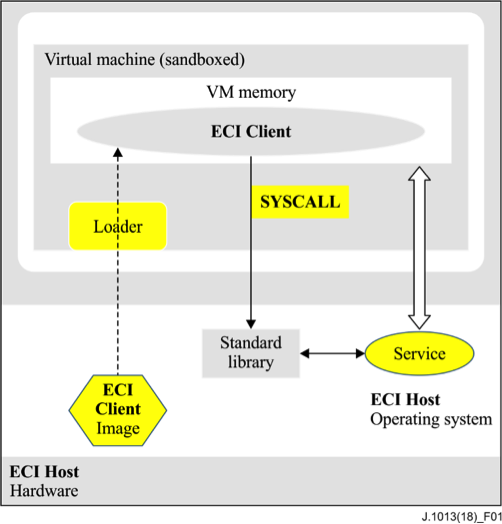
\includegraphics[width=\columnwidth]{Figure1}
\caption{ECI Host - Hardware}\label{fig:fig1} 
\end{figure}
%%======%%

And for a table:
%%= example table =%%
\starttable
\caption{Table title style}\label{tab:tab1} 
\begin{small}
\begin{tabu}{|c|c|}
\hline
 \rowfont{\bfseries}Character & Entity Reference\\ 
  & \\
\hline
\hline
\& & \&amp; \\
\hline
 < & \&lt;\\
 \hline
 > & \&gt; \\
\hline
``  & \&quot; \\
\hline
 ` & \&apos; \\
\hline
\end{tabu}
\end{small}
\end{table}
%%======%%

And an equation:
%%= example equation =%%
\begin{equation}\label{eq:eq1}
PL(D)=PL(D)+10\log 
\end{equation}
%%======%%

\section{Footnotes}
\label{sec:sec7}
Use footnotes sparingly (or not at all!)\ITUfootnote{To obtain the right formatting for the footnotes, use the predefined command \texttt{\textbackslash{ITUfootnote}}}.
To help your readers, avoid using footnotes altogether and include necessary peripheral observations in the text (within parentheses, if you prefer, as in this sentence).\ITUpar


\section{Using references}
\label{sec:sec8}
List and number all bibliographical references at the end of the paper, and refer to them in the text as shown in this sentence \cite{author2021}.\ITUpar

\section{Page numbering}
\label{sec:sec9}
Please number all pages of your paper.\ITUpar

\section{Authoring recommendations}
\label{sec:sec10}
Define abbreviations and acronyms the first time they are used in the text, even if they have already been defined in the abstract.
Abbreviations and acronyms should be avoided in the title. \ITUpar
Units should be expressed as much as possible in international units, and a dot (``.'') should be used to express decimal points (not ``,'').\ITUpar


\section{Conclusion}
\label{sec:sec11}
The main conclusions may be presented in a short final section.\ITUpar


\section*{Acknowledgement}
\label{sec:ackn}
You may list here colleagues, sponsors and financial supporter that you wish to acknowledge.
This section is not required.\ITUpar


%%= bibliography =%%
\printbibliography 
%%======%%

\ITUpar
\section*{Authors}
\label{sec:auth}

\begin{wrapfigure}{l}{0.32\columnwidth} 
    \vspace{-.1in}
    
\includegraphics[width=0.39\columnwidth]{yourphotofilename.jpg} 
\end{wrapfigure}\textbf{First A. Author} Biographies should be limited to one paragraph consisting of the following: sequentially ordered list of degrees, including years achieved; sequentially ordered places of employ concluding with current employment; association with any official journals or conferences; major professional and/or academic achievements, i.e., best paper awards, research grants, etc.; any publication information (number of papers and titles of books published); current research interests; association with any professional associations.\ITUpar

\begin{wrapfigure}{l}{0.32\columnwidth} 
    \vspace{-.1in}
    
\includegraphics[width=0.39\columnwidth]{yourphotofilename.jpg} 
\end{wrapfigure}\textbf{Second A. Author} Biographies should be limited to one paragraph consisting of the following: sequentially ordered list of degrees, including years achieved; sequentially ordered places of employ concluding with current employment; association with any official journals or conferences; major professional and/or academic achievements, i.e., best paper awards, research grants, etc.; any publication information (number of papers and titles of books published); current research interests; association with any professional associations.\ITUpar

\begin{wrapfigure}{l}{0.32\columnwidth} 
    \vspace{-.1in}
    
\includegraphics[width=0.39\columnwidth]{yourphotofilename.jpg} 
\end{wrapfigure}\textbf{Third A. Author} Biographies should be limited to one paragraph consisting of the following: sequentially ordered list of degrees, including years achieved; sequentially ordered places of employ concluding with current employment; association with any official journals or conferences; major professional and/or academic achievements, i.e., best paper awards, research grants, etc.; any publication information (number of papers and titles of books published); current research interests; association with any professional associations.\ITUpar

\end{document}
%%%=========%%%
